
\chapter{Aplicacion en un modelo fisico de laboratorio}

\section{Descripcion del modelo}

Los ensayos que se llevaron a cabo en este trabajo se realizaron en un modelo fisico ubicado en el Laboratorio de Hidraulica [CITAR] de la Facultad de Ciencias Exactas, Fisicas y Naturales (UNC). El modelo es una representacion a escala reducida 1:65 del Dique Los Molinos, ubicado en la provincia Jujuy.
Como se observa en la figura [REFERENCIAR], el dique está constituido por un terraplén de materiales sueltos y dos vertederos, un tramo a nivel fijo (dique fijo), y otro regulado por 4 compuertas, conocido como dique movil. Sobre el margen derecho, se encuentra el canal moderador.

% ELEGIR OTRA IMAGEN POR QUE EN ESTA EL MODELO ESTA EN CONSTRUCCION
\begin{figure}[ht]
\centering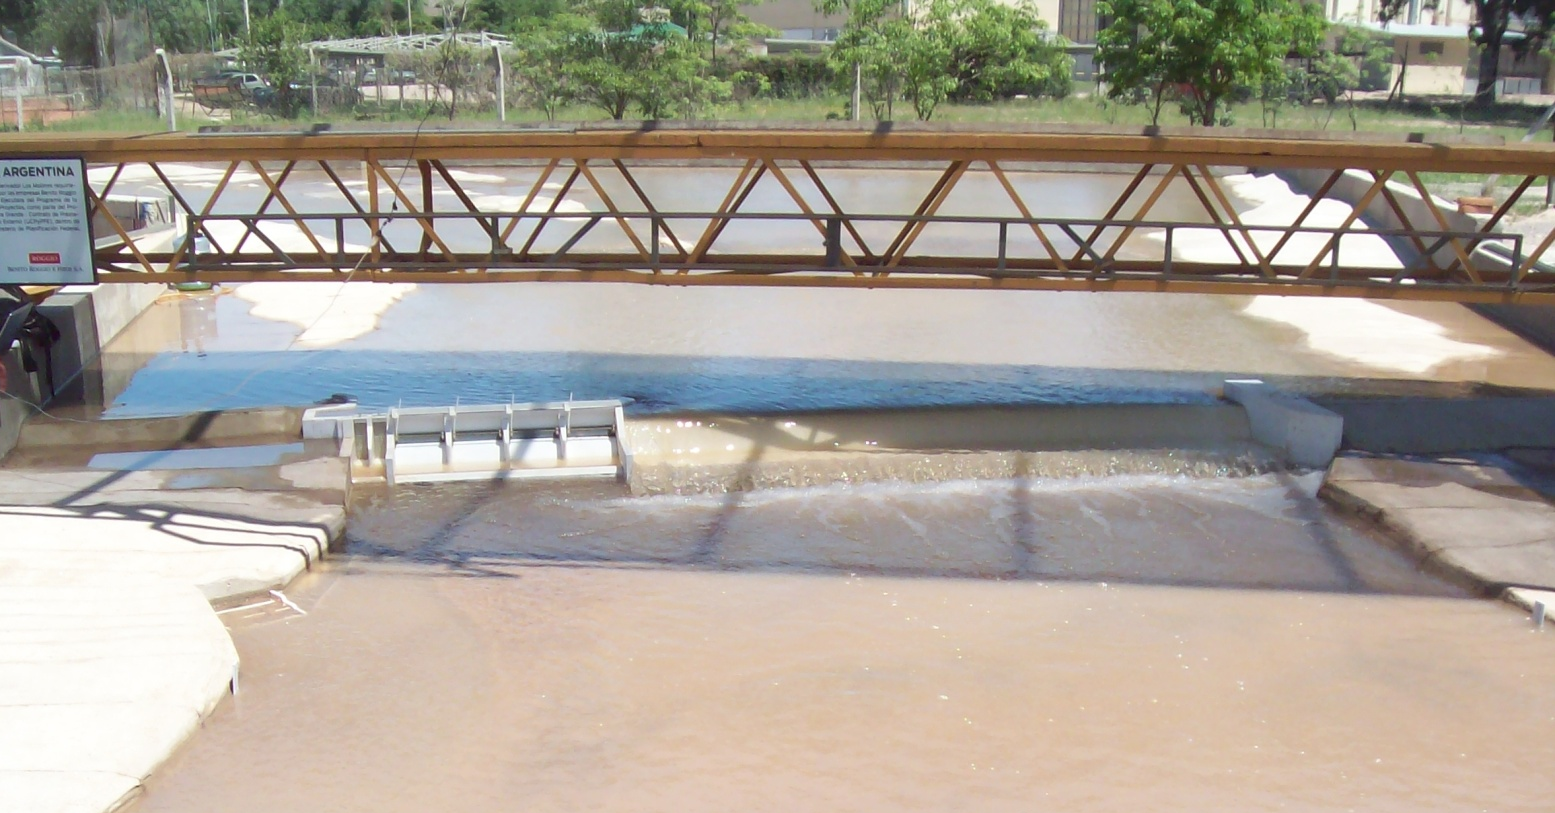
\includegraphics[width=\imsizeS]
{modelo-fisico-dique-los-molinos}
\caption[Modelo fisico dique Los Molinos]{Modelo fisico dique Los Molinos, Laboratorio de Hidráulica, FCEFyN de la UNC.}
\label{fig:modelo-fisico-dique-los-molinos}
\end{figure}

\begin{figure}[ht]
\centering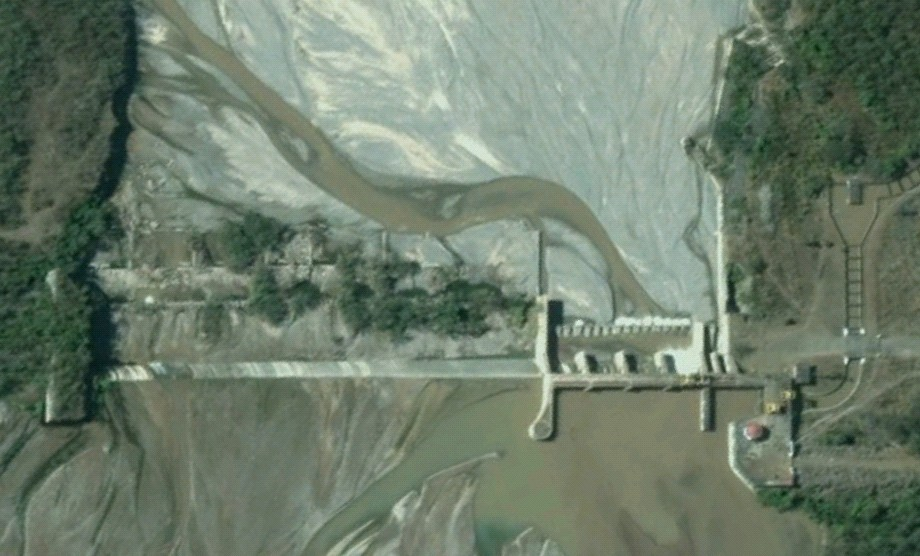
\includegraphics[width=\imsizeS]
{dique-los-molinos}
\caption[Dique Los Molinos]{Dique Los Molinos, Jujuy.}
\label{fig:dique-los-molinos}
\end{figure}

Sobre la zona de interes, se ha construido una plataforma movil que posibilita realizar las mediciones de erosion. Sus componentes principales son : 

\begin{itemize}

\item Un puente grua. Este puede ser trasladado para observar distintas areas del modelo.

\item Una guia-riel y un carro-soporte para la camara Kinect. Ver \ref{fig:sistema-camara-carro}. La guia se anexa al puente grua, lo que permite la translacion de la camara a lo ancho del modelo.

\end{itemize}

\begin{figure}[ht]
\centering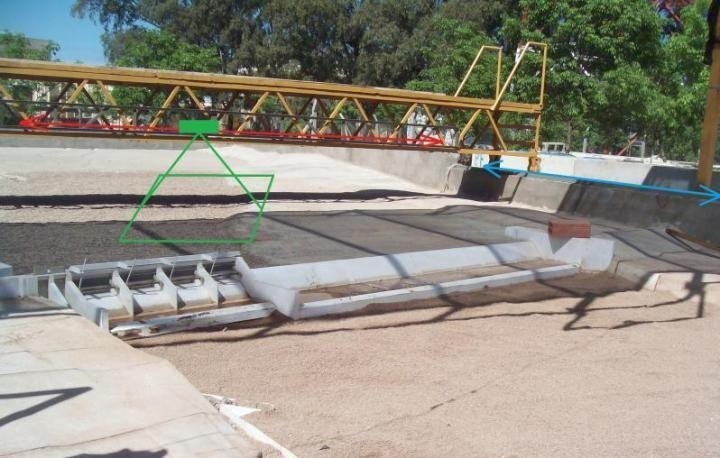
\includegraphics[width=\imsize]
{esquema-camara-puente-grua}
\caption[Puente grua]{Puente grua. Las flechas indican la direcciones en la que se puede transladar la camara (esquematizada con el recuadro verde). En rojo, translacion utilizando el carro soporte, mientras que la trayectoria en azul, se consigue movilizando el puente grua.}
\label{fig:esquema-camara-puente-grua}
\end{figure}

\begin{figure}[ht]
\centering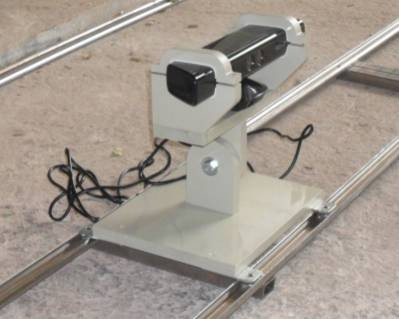
\includegraphics[width=\imsize]
{sistema-camara-carro}
\caption[Sistema camara-soporte]{Soporte construido para trasladar la camara sobre el modelo.}
\label{fig:sistema-camara-carro}
\end{figure}

%%%%%%%%%%%%%%%%%%%%%%%%%%%%%%%%%%%%%%%%%%%%%%%%%%%%%%%%%%%%%%%%%%%%%%%%%%%%%%%

\section{Etapas de un ensayo hidraulico}
\label{sec:etapas-previas-medicion}

Un ensayo hidraulico esta compuesto por las siguientes etapas :  
\begin{enumerate}

\item Nivelacion del material suelto (arena) hasta la cota del terreno medido con la topografia provista. Esto establece la condicion inicial del modelo. Se utilizo una cota media de 1360 m s.n.m. Figura [REFERENCIAR].

\item Encendido del modelo. Se realiza un control del caudal hasta alcanzar el caudal asociado al ensayo.

\item Monitoreo de la erosion durante el ensayo hasta alcanzar la condicion de estabilidad. Estas mediciones se llevan a cabo con nivel optico y mira.

\item Apagado del modelo. Se apaga la bomba hidraulica, se cierran las compuertas correspondientes, y se deja drenar el modelo.

\item Medicion de erosion. 

\end{enumerate}

La tecnica propuesta en este trabajo solo aborda la etapa 5, por lo que no se describe con mas detalles las tareas previas.

%%%%%%%%%%%%%%%%%%%%%%%%%%%%%%%%%%%%%%%%%%%%%%%%%%%%%%%%%%%%%%%%%%%%%%%%%%%%%%%

\section{Metodologia de medicion}

En este seccion, se descibe la aplicacion de la tecnica digital de medicion de erosion. \\

Se tuvieron en cuenta un conjunto de consideraciones que permiten obtener resultados optimos, estas son :

\begin{itemize}

\item La superfie debe estar libre de agua. Como se menciono en \ref{sec:consideraciones-kinect}, objetos con caracteristicas reflectantes afectan al sensor de profundidad de la Kinect. Figura \ref{fig:modelo-condiciones-agua}.

\item La escena debe estar al resguardo de la luz solar, como se explica en \ref{sec:consideraciones-kinect}. Para esto se utilizo un nylon de color negro colocado sobre el puente grua, como se puede observar en las figuras \ref{fig:modelo-lona1} y \ref{fig:modelo-lona2}. Alternativamente, se considero realizar las mediciones al atardecer cuando la luz solar es mas tenue. Se concluyo que utilizando el nylon se obtienen condiciones luminicas estables, sin importar el horario.

\item La guia debe estar horizontalizada. El plano desde el que se captura la escena debe estar a una altitud constante para que la representacion de la superficie sea consistente.

\item La camara debe ubicarse en un rango de 0.4 m a 2m [REVISAR GRAFICO] de la escena para que el error se mantenga dentro del intervalo aceptable \ref{sec:consideraciones-kinect}. EXPLICAR MEJOR.

\end{itemize}

\begin{figure}[h]
\centering
\begin{minipage}[t]{.45\textwidth}
\begin{center}
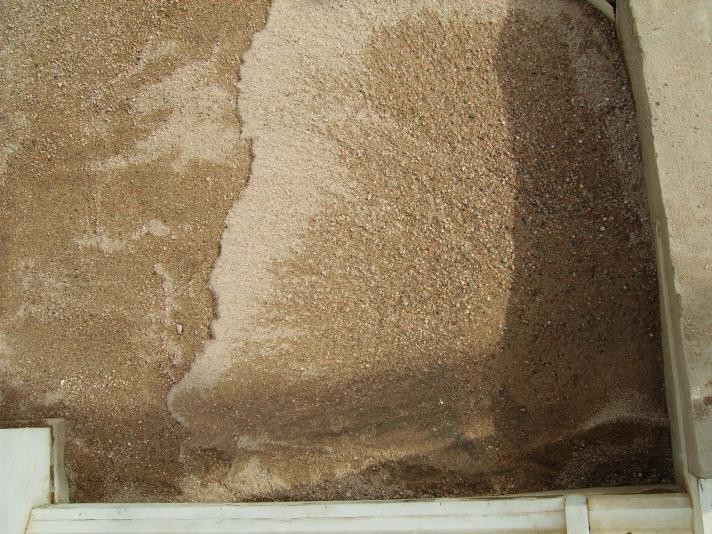
\includegraphics[width=\imsizeS]{modelo-sin-agua} % primera imagen colocada a la izquierda
\end{center}
\end{minipage}
\hfill
\begin{minipage}[t]{.45\textwidth}
\begin{center}
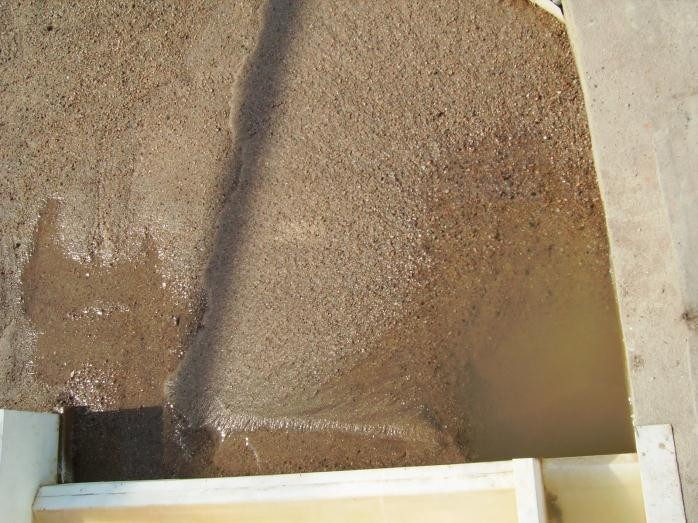
\includegraphics[width=\imsizeS]{modelo-con-agua} % segunda imagen colocada a la derecha
\end{center}
\end{minipage}
\hfill
\caption{A la derecha condicion correcta para la medicion. A la izquiera se observan espejos de agua que interfieren el sensor infrarojo de la camara.}
\label{fig:modelo-condiciones-agua}
\end{figure}

\begin{figure}[ht]
\centering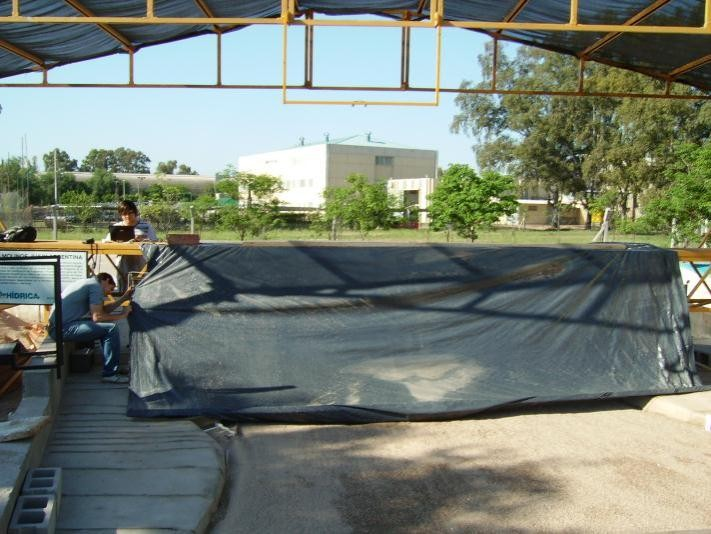
\includegraphics[width=\imsizeS]
{modelo-lona1}
\caption[Modelo cubierto por nylon.]
{Forma de colocar el nylon sobre el puente grua para cubrir todo el largo del riel.}
\label{fig:modelo-lona1}
\end{figure}

\begin{figure}[ht]
\centering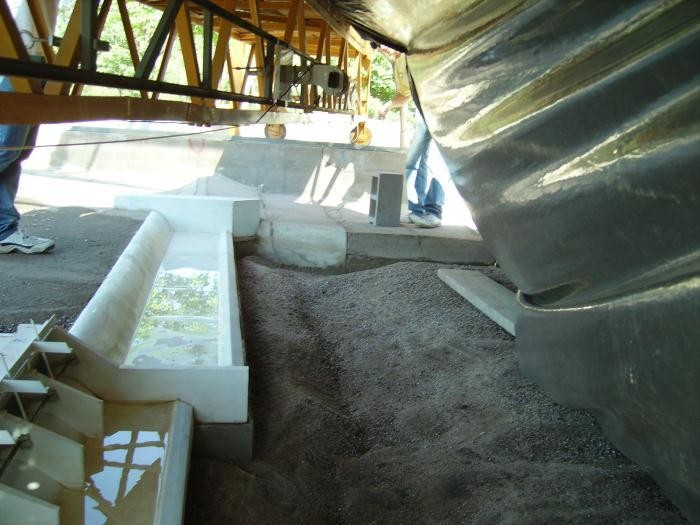
\includegraphics[width=\imsizeS]
{modelo-lona2}
\caption[Sombra generada por nylon sobre el modelo.]
{Sombra producida por el nylon para tomar imagenes sin interferencias.}
\label{fig:modelo-lona2}
\end{figure}

Habiendo verificado las condiciones anteriores, se introduce el carro-soporte en carril y se inicia el software de registracion REFERENCIAR[APLICACION]. \\
 
En la figura \ref{fig:aguas-abajo-desplazamiento-carro}, se observa como manipular la plataforma movil para capturar la escena. El carro se desplaza aproximadamente 40 cm entre cada captura, para que el area sobrelapada entre dos nubes puntos continuas este proxima al 50\%. Como se explica en REFERENCIAR[APLICACION], la aplicacion indica si la captura mas reciente pudo ser registrada, lo que permite correguir la ubicacion del sensor si es necesario.

\begin{figure}[ht]
\centering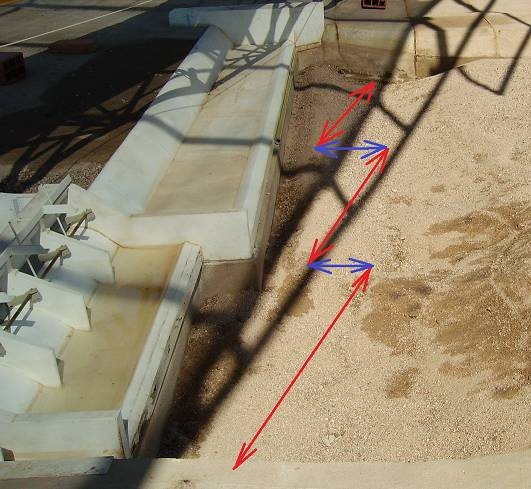
\includegraphics[width=\imsize]
{aguas-abajo-desplazamiento-carro}
\caption[Desplazamiento de la camara]{Recorrido del puente grúa y del carro-soporte sobre la escena. Las flechas rojas indican desplazamiento de la camara y las flechas azules representan el movimiento del puente.}
\label{fig:aguas-abajo-desplazamiento-carro}
\end{figure}

AGREGAR IMAGEN QUE MUESTRE SOBRELAPAMIENTO.

En REFERENCIAR[APLICACION] se describe que para poder realizar la conversion a prototipo es necesario un punto fijo con cota conocida en dicha escala. Con este fin, es recomendable que la escena capture estructuras con medidas de elevacion dada por mediciones topograficas. En caso contrario, se puede medir con nivel optico un punto visible en la escena y utilizar su cota prototipo como referencia.  

%%%%%%%%%%%%%%%%%%%%%%%%%%%%%%%%%%%%%%%%%%%%%%%%%%%%%%%%%%%%%%%%%%%%%%%%%%%%%%%

\section{Ensayos realizados}

AGREGAR TABLA.

\subsection{Medicion de erosion maxima}

En ingenieria civil, este tipo de ensayo tiene como objetivo encontrar cotas maxima de erosion y determinar el nivel de fundacion de los muros del dique. \\ 
Se muestran los mapas 3D en escala prototipo, generados a partir del relevamiento de fosos de erosion ubicados aguas abajo, para 2 ensayos con caudal de 900 m**3/s y 4200 m**3/s, respectivamente. \\

Muro de separacion entre canal moderador y dique movil : 1370,45 m s.n.m.\\

Ensayo 900 m**3/s \\
AGREGAR MAPA 3D RGB \\
%{Foso de erosion aguas abajo del dique movil. Caudal 900 m**3/s. Modelo 3D en colores.}

AGREGAR MAPA 3D ESCALA DE PROFUNDIDAD.\\
%{Foso de erosion aguas abajo del dique movil. Caudal 900 m**3/s. Modelo 3D de elevaciones.}

Ensayo 4200 m**3/s \\
AGREGAR MAPA 3D RGB \\
%{Foso de erosion aguas abajo del dique movil. Caudal 4200 m**3/s. Modelo 3D en colores.}

AGREGAR MAPA 3D ESCALA DE PROFUNDIDAD. \\
%{Foso de erosion aguas abajo del dique movil. Caudal 4200 m**3/s. Modelo 3D de elevaciones.}

AGREGAR PERFILES.\\

%Fecha : 31/10/2012. Caudal :  900 m**3 / s.
%Fecha : 05/11/2012. Caudal : 4200 m**3 / s

\subsection{Medicion de formas de fondo}

En este ensayo se relevan canalizaciones hacia las compuertas del dique movil y el canal moderador, con el objetivo de evaluar la forma de operacion de cada compuerta. El analisis de canales sobre la superficie del modelo requiere una densidad de puntos elevada en grandes areas de superficie. La tecnica digital aborda esta tarea de forma mucha mas eficiente y precisa que la metodologia tradicional. \\
Se muestran los modelos 3D, en escala prototipo, generados a partir del area de modelacion aguas arriba del dique, para un ensayo con caudal de XXX m**3/s.\\
Como punto de referencia se utilizo el muro de encauzamiento a 1377.7 m s.n.m.

AGREGAR MAPA 3D ESCALA DE PROFUNDIDAD. \\
% \begin{figure}[ht]
% \centering\includegraphics[width=\imsize]
% {aguas_arriba_Q600_rgb}
% \caption[Area aguas arriba del dique. Q600. RGB]
% {Area aguas arriba del dique. Q600. RGB.}
% \label{fig:aguas_arriba_Q600_rgb}
% \end{figure}

AGREGAR MAPA 3D ESCALA DE PROFUNDIDAD. \\
% {Area aguas arriba del dique. Caudal XXX m**3/s. Modelo 3D de elevaciones.}

% Fecha : 29/10/2013. Caudal : XXX m**3 / s.
